\documentclass[letter,11pt]{article}

\usepackage[spanish,es-nodecimaldot]{babel}
\usepackage[utf8]{inputenc}

\usepackage{lmodern}
\usepackage[T1]{fontenc}
\usepackage{textcomp}

\usepackage{framed}
\usepackage[svgnames]{xcolor}
\colorlet{shadecolor}{Gainsboro!50}

\usepackage{graphicx}
\usepackage{pstricks}

\usepackage{anysize}
\marginsize{3cm}{2cm}{2cm}{3cm}

\usepackage{siunitx}
\usepackage{amsmath}
\usepackage{array}

\usepackage{fancyhdr}
\usepackage{lastpage}
\pagestyle{fancy}
\fancyhf{}
\fancyhead[LE,RO]{Física Básica III}
\fancyfoot[CO,CE]{\thepage\ de \pageref{LastPage}}

\special{papersize=215.9mm,279.4mm}

\usepackage[
    pdfauthor={Carlos Eduardo Caballero Burgoa},%
    pdftitle={Física Básica III},%
    pdfsubject={2do Parcial},%
    colorlinks,%
    citecolor=black,%
    filecolor=black,%
    linkcolor=black,%
    urlcolor=black,
    breaklinks]{hyperref}
\usepackage{breakurl}

\newcommand{\blankpage}{
\newpage
\thispagestyle{empty}
\mbox{}
\newpage
}

\renewcommand{\arraystretch}{1.2}

\begin{document}

\begin{center}
    {\Large \bf{Segundo parcial}}
\end{center}

\noindent\fbox{%
    \parbox{\textwidth}{%
        Estudiante: CABALLERO BURGOA, Carlos Eduardo \\
        Carrera: Ingeniería Electromecánica \\
        Correo: cijkb.j@gmail.com
    }%
}

\vspace{0.5cm}

\begin{enumerate}
\item La diferencia de potencial en las terminales de una batería es de
$8.4 [V]$ cuando en esta hay una corriente de $1.5 [A]$ de la terminal negativa
a la positiva. Cuando la corriente es de $3.5 [A]$ en la dirección inversa, la
diferencia de potencial es de $10.20 [V]$. ¿Cuál es la FEM de la batería?

\begin{itemize}
    \item $ 7.45 [V]$.
    \item \textcolor{red}{$ 8.94 [V]$.}
    \item $ 9.26 [V]$.
    \item $10.02 [V]$.
\end{itemize}

\textbf{Solución:}

Considerando la ecuación:

\begin{equation*}
    V_{ab} = \mathcal{E}-RI
\end{equation*}

Por tanto:

\begin{equation*}
    \begin{cases}
        8.4 = \mathcal{E}-1.5R & \text{descarga de la batería} \\
        10.2 = \mathcal{E}+3.5R & \text{carga de la batería}
    \end{cases}
\end{equation*}

\begin{equation*}
    \mathcal{E} = 8,94 [V]
\end{equation*}

\item Dos focos de $120 [V]$, una de $25 [W]$ y otra de $200 [W]$, se conectaron
en serie a través de una línea de $240 [V]$, pero se quemó de inmediato ...

\begin{itemize}
    \item \textcolor{red}{El de $25 [W]$.}
    \item El de $200 [W]$.
    \item Se quemaron los dos.
    \item Ninguno se quemó.
\end{itemize}

\textbf{Solución:}

Sabiendo que:

\begin{equation*}
    P = I\,V
\end{equation*}

Es posible calcular la corriente soportada por cada bombilla:

\begin{equation*}
    I_1 = \frac{P_1}{V} = 0.2083 [A]
\end{equation*}
\begin{equation*}
    I_2 = \frac{P_2}{V} = 1.6667 [A]
\end{equation*}

Al estar en serie en un circuito de $240 [V]$, se puede calcular la corriente
del circuito:

\begin{equation*}
    240 = \frac{P_1}{I}+\frac{P_2}{I}
        = \frac{P_1+P_2}{I}
\end{equation*}
\begin{equation*}
    I = \frac{P_1+P_2}{240} = 0,9375 [A]
\end{equation*}

Por tanto el primer foco se quemó

\item Calcule la corriente que fluye por el amperímetro $A$ (de resistencia
interna igual a cero).

\begin{figure}[!h]
\centering
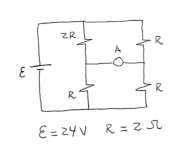
\includegraphics[scale=2.00]{resources/q3.eps}
\end{figure}

\begin{itemize}
    \item $0.0  [A]$.
    \item $0.86 [A]$.
    \item \textcolor{red}{$1.71 [A]$.}
    \item $2.06 [A]$.
\end{itemize}

\textbf{Solución:}

\begin{figure}[!h]
\centering
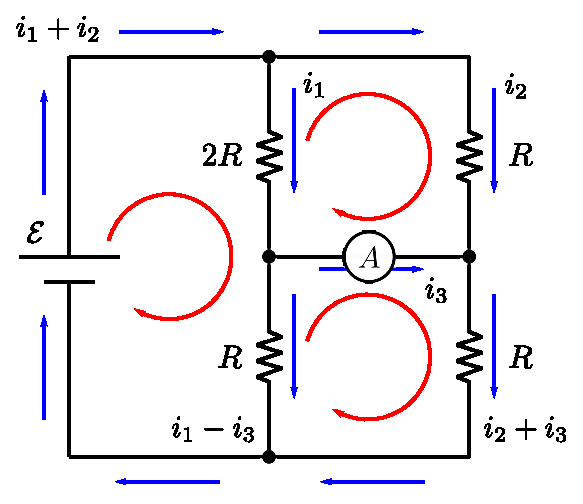
\includegraphics[scale=0.76]{resources/a3.eps}
\end{figure}

Usando la regla de nodos:

\begin{equation*}
    \begin{cases}
        24-4i_1-2(i_1-i_3) = 0 \\
        -2i_2+4i_1 = 0 \\
        -2(i_2+i_3)+2(i_1-i_3) = 0
    \end{cases}
\end{equation*}

Resolviendo el sistema de ecuaciones, se obtiene:

\begin{equation*}
    \begin{cases}
        i_1 = 3.4286 [A] \\
        i_2 = 6.8571 [A] \\
        i_3 = -1.7143 [A]
    \end{cases}
\end{equation*}

\item Cierta batería de automóvil ($12 [V]$) puede proporcionar una carga total
de $125 [Ah]$ (amperio-horas) antes de agotarse. Suponiendo que la diferencia de
potencial entre las terminales permanece constante, ¿Cuánto tiempo puede
suministrar energía con una potencia de $110 [W]$?

\begin{itemize}
    \item \textcolor{red}{$13.64 [h]$.}
    \item $14.08 [h]$.
    \item $15.39 [h]$.
    \item $16.47 [h]$.
\end{itemize}

\textbf{Solución:}

Se calcula la corriente con la ecuación:

\begin{equation*}
    P = I\,V
\end{equation*}
\begin{equation*}
    I = \frac{P}{V} = \frac{110}{12} = 9.1667 [A]
\end{equation*}

Por tanto el tiempo es:

\begin{equation*}
    t = \frac{125 [Ah]}{9.1667 [A]} = 13.6354 [h]
\end{equation*}

\item La función de la fuerza electromotriz en un circuito consiste en:

\begin{itemize}
    \item Suministrar electrones al circuito.
    \item \textcolor{red}{Elevar el potencial de los electrones.}
    \item Disminuir el potencial de los electrones.
    \item Aumentar la rapidez de los electrones.
\end{itemize}

\textbf{Solución:}

Los electrones se mueven, cuando hay un camino disponible, desde un punto de
exceso de electrones (energía potencial más alta) a un punto deficiente en
electrones (energía potencial más baja).

La fuerza que provoca este movimiento es la fuerza electromotriz.

\item Un calentador (estufa) que opera con una línea de $120 [V]$, tiene una
resistencia de $14 [\Omega]$. ¿Cuánto cuesta hacer funcionar durante
$6 [h] 25 [min]$, si se paga $5.22 [Bs]$ el kWh (kilovatio-hora)?

\begin{itemize}
    \item $30.08 [Bs]$.
    \item $32.19 [Bs]$.
    \item \textcolor{red}{$34.45 [Bs]$.}
    \item $36.27 [Bs]$.
\end{itemize}

\textbf{Solución:}

Se calcula el potencial eléctrico con la ecuación:

\begin{equation*}
    P = \frac{V^2}{R} = \frac{(120)^2}{14} = 1028.57 [W] = \frac{36}{35} [kW]
\end{equation*}

El consumo es:

\begin{equation*}
    \frac{36}{35} \left(6+\frac{25}{60}\right) = \frac{33}{5} [kWh]
\end{equation*}

Por tanto, el costo es:

\begin{equation*}
    \frac{33}{5}\,5.22 = 34.452 [Bs]
\end{equation*}

\item Calcule el potencial del punto $a$ con respecto al punto $b$. Todas las
resistencias están en ohmios y todas las FEM en voltios.

\begin{figure}[!h]
\centering
\includegraphics[scale=1.80]{resources/q7.eps}
\end{figure}

\begin{itemize}
    \item $ 0.11 [V]$.
    \item \textcolor{red}{$ 0.22 [V]$.}
    \item $-0.67 [V]$.
    \item $10.22 [V]$.
\end{itemize}

\textbf{Solución:}

\begin{figure}[!h]
\centering
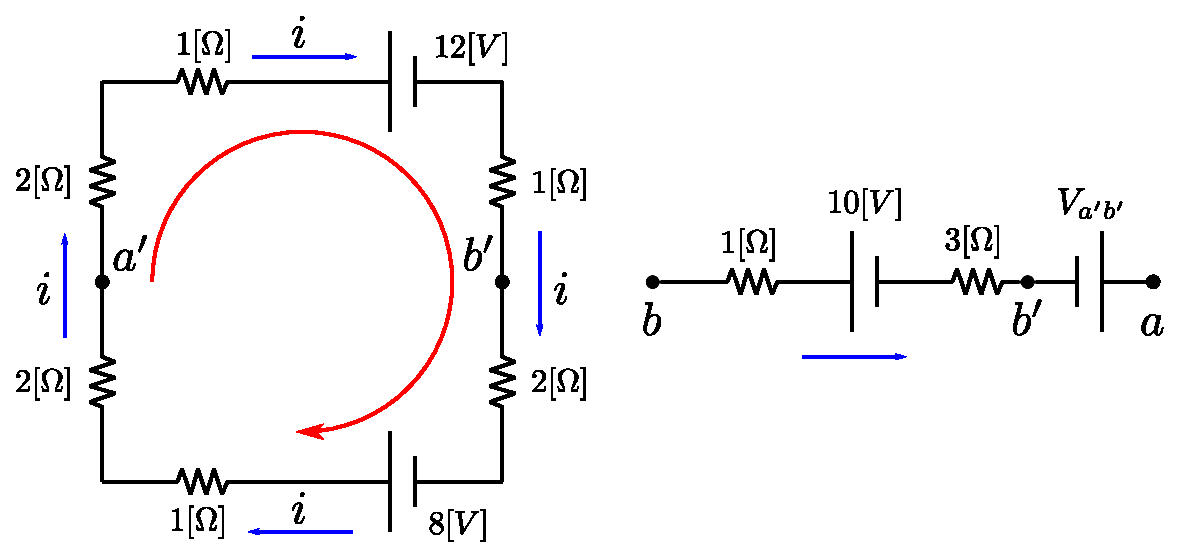
\includegraphics[scale=0.64]{resources/a7.eps}
\end{figure}

Calculando la corriente en la malla:

\begin{equation*}
    -2i-1i-12-1i-2i+8-1i-2i = 0
\end{equation*}
\begin{equation*}
    -9i-4 = 0
\end{equation*}
\begin{equation*}
    i = -\frac{4}{9}[A]
\end{equation*}

Calculando el potencial entre $a'$ y $b'$:

\begin{equation*}
    V_{a'b'} = -2\left(\frac{4}{9}\right)
               + 8-1\left(\frac{4}{9}\right)
               - 2\left(\frac{4}{9}\right)
             = 10.22 [V]
\end{equation*}

Por tanto el potencial $V_{ab}$ es:

\begin{equation*}
    V_{ab} = 0-10+0+10.22 = 0.22 [V]
\end{equation*}

\item Calcule $V_b - V_a$, la diferencia de potencial de $b$ respecto de $a$.

\begin{figure}[!h]
\centering
\includegraphics[scale=2.00]{resources/q8.eps}
\end{figure}

\begin{itemize}
    \item $ 4.20 [V]$.
    \item \textcolor{red}{$-3.60 [V]$.}
    \item $ 2.35 [V]$.
    \item $-1.18 [V]$.
\end{itemize}

\textbf{Solución:}

\begin{figure}[!h]
\centering
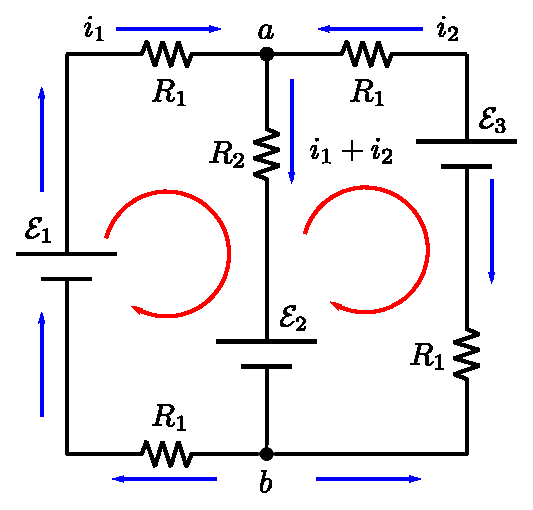
\includegraphics[scale=0.74]{resources/a8.eps}
\end{figure}

De la regla de las mallas, definimos:

\begin{equation*}
    \mathcal{E}_1-R_1i_1-R_2(i_1+i_2)-\mathcal{E}_2-R_1i_1 = 0
\end{equation*}
\begin{equation*}
    \mathcal{E}_1-\mathcal{E}_2-(2R_1+R_2)i_1-R_2i_2 = 0
\end{equation*}
\begin{equation*}
    R_1i_2-\mathcal{E}_3+R_1i_2+\mathcal{E}_2+R_2(i_1+i_2) = 0
\end{equation*}
\begin{equation*}
    \mathcal{E}_2-\mathcal{E}_3+R_2i_1+(2R_1+R_2)i_2 = 0
\end{equation*}
\begin{equation*}
    \begin{cases}
        4.7i_1+2.3i_2 = -1.8 \\
        2.3i_1+4.7i_2 = 1.2
    \end{cases}
\end{equation*}

Los corrientes son:

\begin{equation*}
    \begin{cases}
        i_1 = -\dfrac{187}{280} \\
        \\
        i_2 = \dfrac{163}{280}
    \end{cases}
\end{equation*}

Por tanto, $V_{ba}$ es:

\begin{equation*}
    V_{ba} = -R_2(i_1+i_2)-\mathcal{E}_2 = -3.6028 [V]
\end{equation*}

\item Un capacitor de $2 [\mu F]$ inicialmente descargado se conecta en serie
con un resistor de $6000 [\Omega]$ y una fuente de FEM de $90 [V]$. El circuito
se cierra en $t = 0 [s]$. ¿En qué instante la tasa a la que la energía eléctrica
(potencia) se disipa en el resistor es igual a la tasa a la cual la energía
eléctrica se almacena en el capacitor?

\begin{itemize}
    \item $4.58 [ms]$.
    \item $5.97 [ms]$.
    \item $7.23 [ms]$.
    \item \textcolor{red}{$8.32 [ms]$.}
\end{itemize}

\textbf{Solución:}

La tasa instantánea a la que la energía eléctrica se disipa en el resistor es:

\begin{equation*}
    P_R = \frac{i^2}{R}
\end{equation*}

y la tasa a la que la energía se almacena en el capacitor es:

\begin{equation*}
    P_C = \frac{iq}{C}
\end{equation*}

Igualando ambas ecuaciones:

\begin{equation*}
    P_R = P_C
\end{equation*}
\begin{equation*}
    \frac{i^2}{R} = \frac{iq}{C}
\end{equation*}
\begin{equation*}
    \frac{q}{RC} = I
\end{equation*}

La carga del capacitor esta dada por la ecuación:

\begin{equation*}
    q = Q_f\,(1-e^{-t/RC}) = C\mathcal{E}\,(1-e^{-t/RC})
\end{equation*}

y la corriente eléctrica es:

\begin{equation*}
    i = I_o\,e^{-t/RC} = \frac{\mathcal{E}}{R}\,e^{-t/RC}
\end{equation*}

Uniendo todas las ecuaciones:

\begin{equation*}
    \dfrac{C\mathcal{E}\,(1-e^{-t/RC})}{RC} = \frac{\mathcal{E}}{R}\,e^{-t/RC}
\end{equation*}
\begin{equation*}
    1-e^{-t/RC} = e^{-t/RC}
\end{equation*}
\begin{equation*}
    2e^{-t/RC} = 1
\end{equation*}
\begin{equation*}
    e^{-t/RC} = 0.5
\end{equation*}
\begin{equation*}
    -\frac{t}{RC} = ln(0.5)
\end{equation*}
\begin{equation*}
    t = -RC\,ln(0.5) = \num{8.3178e-3} [s]
\end{equation*}

\end{enumerate}

\end{document}

